\clearpage
\section{Vorhersage der Dynamik durch das Fernfeld}
\label{sec:exp_unblur}
Bei der Durchführung von in vitro Experimenten mit Herzen gibt es verschiedene Möglichkeiten, die Messung der elektrischen Erregung auf der Herzoberfläche durchzuführen. Zum einen können Elektroden zur Messung benutzt werden, zum anderen können auch Fluoreszenzmessungen durchgeführt werden. Bei der Verwendung von Elektroden wird effektiv nicht das unmittelbare elektrische Feld auf der Herzoberfläche sondern ein Fernfeld dessen gemessen. Es stellt sich nun die Frage, ob aus der Kenntnis dieses Fernfeldes die korrekte Erregung auf der Oberfläche bestimmt werden kann. Eine experimentelle Untersuchung dieser Fragestellung wird im Folgenden durchgeführt. Hierfür müssen zuerst diese Fernfeldaufnahmen für das \textit{Barkley}- und für das \textit{Mitchell-Schaeffer}-Modell erzeugt werden. Das Fernfeld wird dabei nicht korrekt simuliert, sondern durch eine gaußsche Unschärfe nachgebildet. Im Folge dessen wird auf das gesamte Feld der Spannungsvariable beider Modelle eine solche Unschärfe mit einer Breite $\sigma_{Blur} = 8.0$ mittels einer Faltung angewendet. Eine exemplarische Darstellung des emulierten Fernfeldes und des tatsächlichen Feldes ist in Abbildungen \ref{fig:exp_unblur_barkley} und \ref{fig:exp_unblur_mitchell_schaeffer} zu finden.

\begin{figure}[h]
	\centering
	\begin{subfigure}{.5\textwidth}
		\centering
		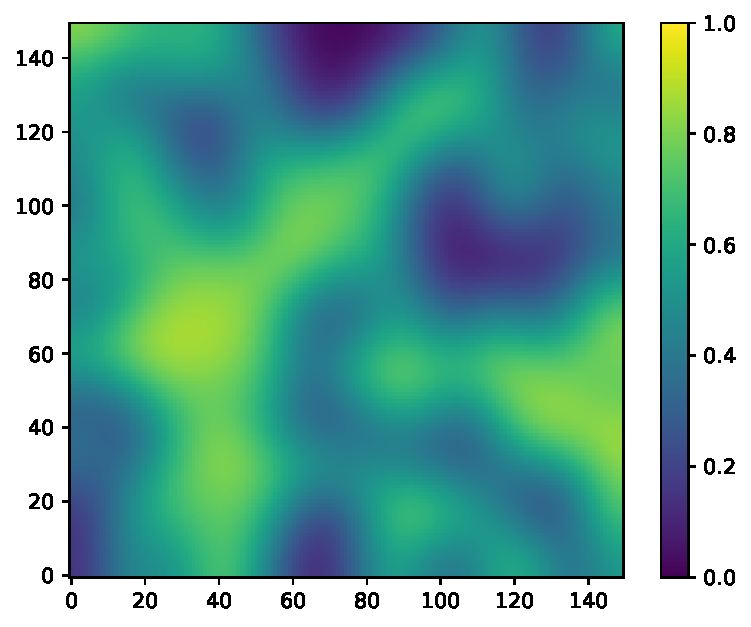
\includegraphics[height=2.5in]{figures/results/unblur/barkley_u_blur_blured.pdf}
		\setcapmargin[1cm]{1cm}
		\caption{Emuliertes Fernfeld}
		\label{fig:exp_unblur_barkley_blurred}
	\end{subfigure}%
	\begin{subfigure}{.5\textwidth}
		\centering
		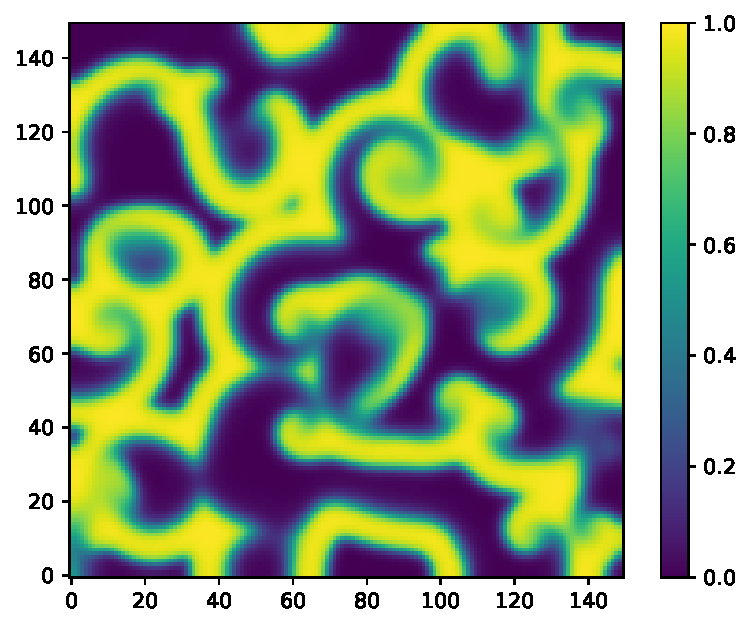
\includegraphics[height=2.5in]{figures/results/unblur/barkley_u_blur_orig.pdf}
		\setcapmargin[1cm]{1cm}
  		\caption{Echte Erregung des Modells}
  		\label{fig:exp_unblur_barkley_orig}
	\end{subfigure}
	\caption{Graphische Darstellung der $u$-Variable des \textit{Barkley}-Modells. Links ist das emulierte Fernfeld und rechts das tatsächliche $u$-Feld des Modells zu sehen.}
	\label{fig:exp_unblur_barkley}
\end{figure} 

\begin{figure}[h]
	\centering
	\begin{subfigure}{.5\textwidth}
		\centering
		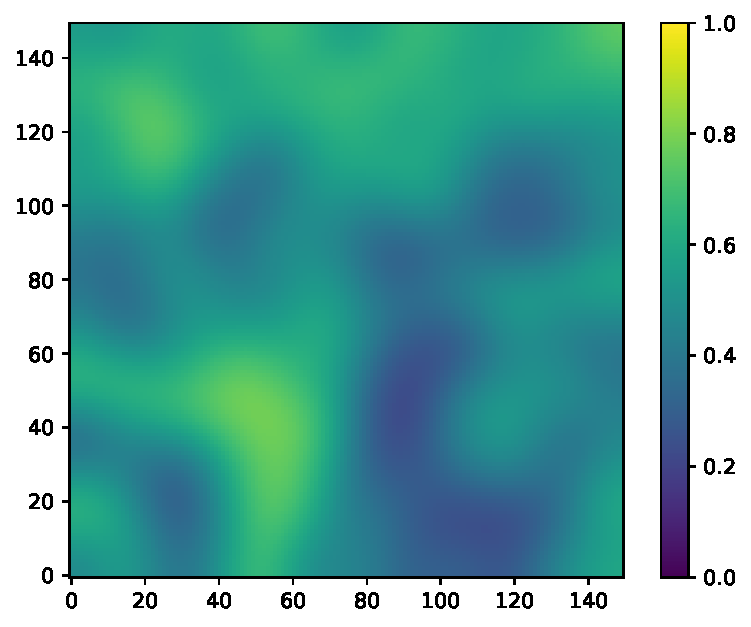
\includegraphics[height=2.5in]{figures/results/unblur/mitchell_v_blur_blured.pdf}
		\setcapmargin[1cm]{1cm}
		\caption{Emuliertes Fernfeld}
		\label{fig:exp_unblur_mitchell_schaeffer_blurred}
	\end{subfigure}%
	\begin{subfigure}{.5\textwidth}
		\centering
		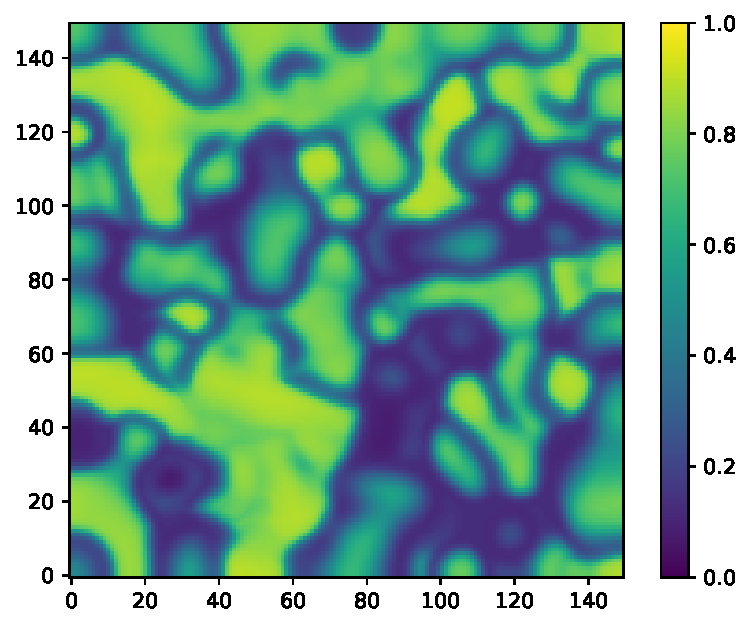
\includegraphics[height=2.5in]{figures/results/unblur/mitchell_v_blur_orig.pdf}
		\setcapmargin[1cm]{1cm}
  		\caption{Echte Erregung des Modells}
  		\label{fig:exp_unblur_mitchell_schaeffer_orig}
	\end{subfigure}
	\caption{Graphische Darstellung der $v$-Variable des \textit{Mitchell-Schaeffer}-Modells. Links ist das emulierte Fernfeld und rechts das tatsächliche $v$-Feld des Modells zu sehen.}
	\label{fig:exp_unblur_mitchell_schaeffer}
\end{figure} 

\FloatBarrier
\subsection{Nächste Nachbar Vorhersage}
Zuerst wird diese Aufgabe erneut mit dem \textsc{NN}-Ansatz betrachtet. Die besten gefundenen Hyperparameter dafür sind in Tabelle \ref{tab:exp_unblur_nn_results} aufgelistet. Bemerkenswert ist erneut die geringe Gesamtlaufzeit dieses Ansatzes. Dies wird durch die verhältnismäßig geringe Dimensionalität des Eingabevektors begünstigt. Allerdings sind die Fehlerwerte sehr hoch, sodass die Vorhersage nur geringfügig besser ist als eine Schätzung mit dem Mittelwert als Vorhersage, wie an dem NRMSE $\approx 1.0$ ersichtlich ist.

\begin{table}[h]
	\centering

	\begin{tabular}{ccc}
		\hline		
		\multicolumn{1}{c}{} & Barkley & Mitchell-Schaeffer \\ 
		\hline 
		\rule[-1ex]{0pt}{2.5ex} $\sigma$ & $1$ & $1$ \\ 
		\rule[-1ex]{0pt}{2.5ex} $\Delta \sigma$ & $1$ & $1$ \\ 
		\rule[-1ex]{0pt}{2.5ex} $\delta$ & $4$ & $3$ \\ 
		\rule[-1ex]{0pt}{2.5ex} k & $5$ & $5$ \\ 
		\rule[-1ex]{0pt}{2.5ex} Laufzeit [s] & $53$ & $42$ \\ 
		\rule[-1ex]{0pt}{2.5ex} \textbf{MSE} & \textbf{0.10089} & \textbf{0.06452} \\ 
		\rule[-1ex]{0pt}{2.5ex} \textbf{NRMSE} & \textbf{0.8308} & \textbf{0.9737} \\ 
		\hline 
	\end{tabular} 

	\caption{Ermittelte Hyperparameter der \textit{Nächsten-Nachbar}-Vorhersage für das \textit{Mitchell-Schaeffer}- und das \textit{Barkley}-Modell, welche zu den geringsten Fehlern führen.}
\label{tab:exp_unblur_nn_results}
\end{table} 


\FloatBarrier
\subsection{Radiale Basisfunktionen}
Im Folgenden sind nun die radialen Basisfunktionen ebenfalls auf das Problem angewendet worden. Die dabei gefundenen Hyperparameter sind in Tabelle \ref{tab:exp_unblur_rbf_results} präsentiert. Die optimalen Werte für $\sigma$ und $\Delta \sigma$ sind nicht mit denen des \textsc{NN}-Ansatzes identisch.

\begin{table}[h]
	\centering

	\begin{tabular}{ccc}
		\hline
		\multicolumn{1}{c}{} & Barkley & Mitchell-Schaeffer \\ 
		\hline 
		\rule[-1ex]{0pt}{2.5ex} $\sigma$ & $3$ & $5$ \\ 
		\rule[-1ex]{0pt}{2.5ex} $\Delta \sigma$ & $1$ & $2$ \\ 
		\rule[-1ex]{0pt}{2.5ex} $\delta$ & $3$ & $3$ \\ 
		\rule[-1ex]{0pt}{2.5ex} $\sigma_{RBF}$ & $5.0$ & $9.0$ \\ 
		\rule[-1ex]{0pt}{2.5ex} Laufzeit [s] & $1840$ & $1842$ \\ 
		\rule[-1ex]{0pt}{2.5ex} \textbf{MSE} & \textbf{0.03984} & \textbf{0.03384} \\ 
		\rule[-1ex]{0pt}{2.5ex} \textbf{NRMSE} & \textbf{0.5170} & \textbf{0.7052} \\ 
		\hline 
	\end{tabular} 
	\caption{Ermittelte Hyperparameter der radialen Basisfunktionen für das \textit{Mitchell-Schaeffer}- und das \textit{Barkley}-Modell, welche zu den geringsten Fehlern führen.}
	\label{tab:exp_unblur_rbf_results}
\end{table} 


\FloatBarrier
\subsection{Echo State Network}
Nachdem die klassischen Methoden bereits auf dieses Problem angewendet worden sind, kann es mittels der \textsc{ESN}s erneut betrachtet werden. Hierfür sind die verwendeten Hyperparameter erneut nach Abschnitt \ref{sec:exp_general_esn} gesucht worden. Die Ergebnisse sind in Tabelle \ref{tab:exp_unblur_esn_results} zu finden. Auffällig ist hierbei, dass die optimale Größe $N$ des Reservoirs für beide Modelle unter der maximal betrachteten Größe $N \leq 400$ liegt. Dies kann ein Anzeichen dafür sein, dass für das Bewältigen der Aufgabe kein ausgeprägtes Langzeitgedächtnis vorhanden sein muss, da diese nach Abschnitt \ref{sc:esn} mit der Größe $N$ des Reservoirs skaliert. 
\improvement{Add more details on:long time memory vs N dependency in theory.}

\begin{table}[h]
	\centering
	\captionsetup{width=0.9\linewidth}
	\begin{tabular}{ccc}
		\hline		
		\multicolumn{1}{c}{} &  Barkley & Mitchell-Schaeffer \\ 
		\hline
		\rule[-1ex]{0pt}{2.5ex} $\sigma$ & $7$ & $7$ \\ 
		\rule[-1ex]{0pt}{2.5ex} $\Delta \sigma$ & $1$ & $1$ \\ 
		\rule[-1ex]{0pt}{3.5ex} $N$ & $200$ & $50$ \\ 
		\rule[-1ex]{0pt}{3.5ex} $\rho(|\mathbf{W}|)$ & $1.50$ & $0.10$\\ 
		\rule[-1ex]{0pt}{3.5ex} $\alpha$ & $0.20$ & $0.05$ \\ 
		\rule[-1ex]{0pt}{3.5ex} $\epsilon$ & $0.1$ & $0.1$ \\ 
		\rule[-1ex]{0pt}{3.5ex} $\nu_{max}$ & $\num{1e-5}$ & $\num{1e-4}$\\ 
		\rule[-1ex]{0pt}{3.5ex} $\lambda$ & $\num{5e-10}$ & $\num{5e-6}$\\ 
		\rule[-1ex]{0pt}{2.5ex} Laufzeit [s] & $1603$ & $1540$ \\ 
		\rule[-1ex]{0pt}{2.5ex} \textbf{MSE} & \textbf{0.02443} & \textbf{0.02645} \\ 
		\rule[-1ex]{0pt}{2.5ex} \textbf{NRMSE} & \textbf{0.4048} & \textbf{0.6234} \\ 
		\hline 
	\end{tabular} 
	\caption{Ermittelte Hyperparameter des \textsc{ESN} für das \textit{Mitchell-Schaeffer}- und das \textit{Barkley}-Modell, welche zu den geringsten Fehlern führen.}
	\label{tab:exp_unblur_esn_results}
\end{table}

\FloatBarrier
\subsection{Vergleich}
Zusammenfassend können nun die Ergebnisse der drei Ansätze abermals verglichen werden. Eine vergleichende Übersicht darüber ist in Tabelle \ref{tab:exp_unblur_comparison_results} zu finden. Auch dazu lässt sich erneut sagen, dass die \textsc{ESN}s die geringsten Fehlerwerte erzeugen, doch der \textsc{NN}-Ansatz deutlich schneller berechnet werden kann, sofern sowohl die Laufzeit der Trainings- als auch der Vorhersagephase berücksichtigt werden.\\
Zusätzlich zu der Tabelle ist noch ein exemplarischer grafischer Vergleich der Resultate der drei Ansätze mit der Zielvariable in Abbildung \ref{fig:exp_unblur_barkley_result} dargestellt. Die analoge Darstellung für das \textit{Mitchell-Schaeffer}-Modell ist in Abbildung \ref{fig:apx_unblur_mitchell_result} dargestellt. Es fällt auf, dass die Vorhersage des \textsc{NN}-Ansatzes sogar die Struktur der Dynamik kaum korrekt auflöst. Im Vergleich dazu ist die Vorhersage des \textsc{RBF}-Ansatzes und des \textsc{ESN} deutlich feiner und beinhaltet die Makrostruktur der Dynamik. Des Weiteren ist zu bemerken, dass diese mit dem \textsc{ESN} etwas feiner aufgelöst worden ist, als mit \textsc{RBF}-Ansatz. Zwar stimmen hier auch nicht die feinen Details der Dynamik mit dem Original überein, jedoch ist eine starke Verbesserung im Vergleich zu dem nachgebildeten Fernfeld zu bemerken. Unter Umständen wäre es für zukünftige Arbeiten bei dieser Aufgabe angebracht, eine andere Fehlermetrik als die mittlere quadratische Abweichung zu benutzen, welche die Ähnlichkeit zwischen den Strukturen der Felder stärker berücksichtigt. 

\begin{figure}[h]
	\centering
	\begin{subfigure}{.5\textwidth}
		\centering
		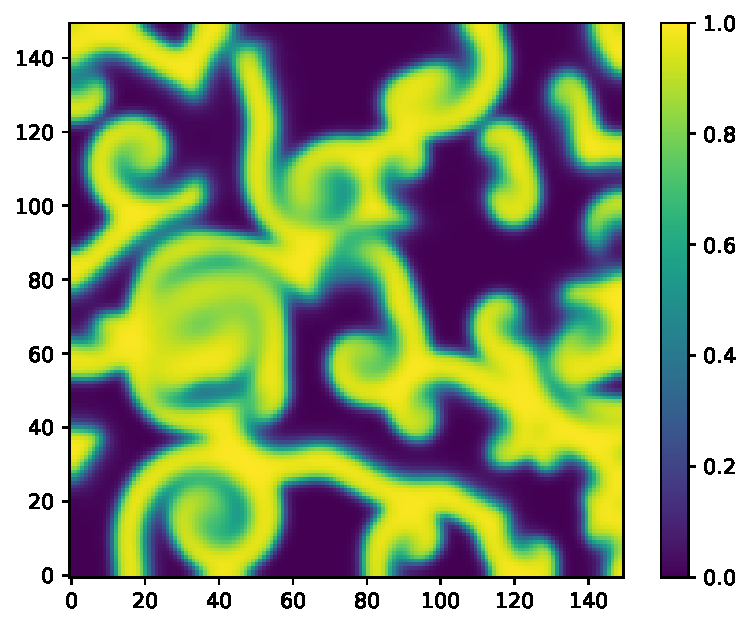
\includegraphics[height=2.5in]{figures/results/unblur/esn_barkley_u_blur_orig.pdf}
		\setcapmargin[1cm]{0.5cm}
		\caption{Echte Erregung des Modells}
		\label{fig:exp_unblur_barkley_result_orig}
	\end{subfigure}%
	\begin{subfigure}{.5\textwidth}
		\centering
		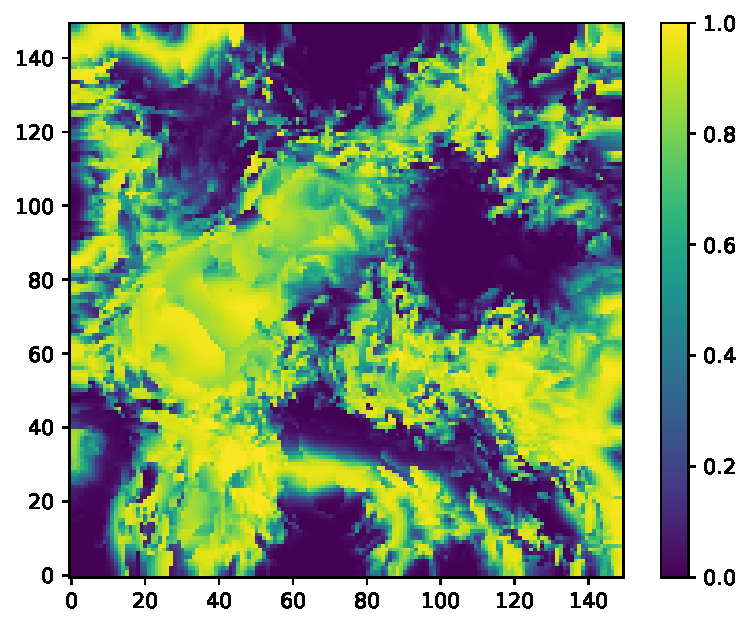
\includegraphics[height=2.5in]{figures/results/unblur/nn_barkley_u_blur_pred.pdf}
		\setcapmargin[1cm]{0.5cm}
  		\caption{Vorhersage des \textsc{NN}-Ansatzes}
  		\label{fig:exp_unblur_barkley_result_nn_pred}
	\end{subfigure}
	\begin{subfigure}{.5\textwidth}
		\centering
		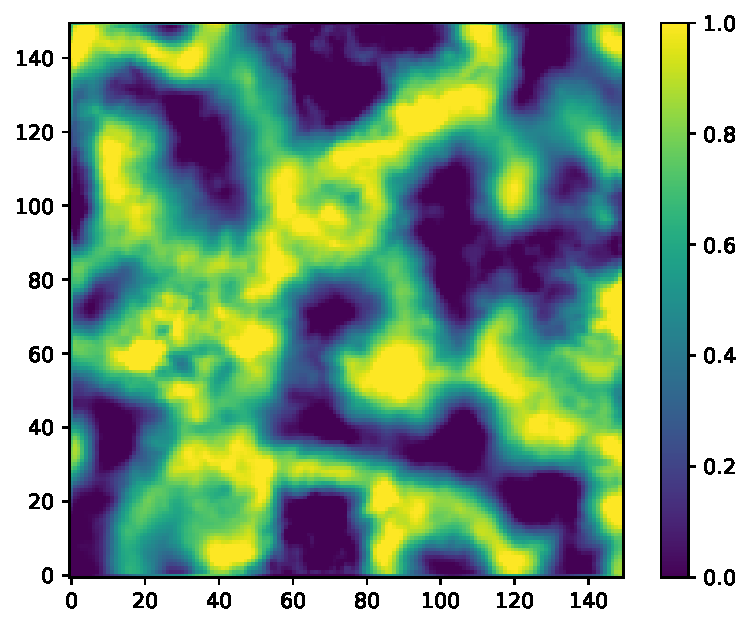
\includegraphics[height=2.5in]{figures/results/unblur/rbf_barkley_u_blur_pred.pdf}
		\setcapmargin[1cm]{0.5cm}
  		\caption{Vorhersage des \textsc{RBF}-Ansatzes}
  		\label{fig:exp_unblur_barkley_result_rbf_pred}
	\end{subfigure}%
	\begin{subfigure}{.5\textwidth}
		\centering
		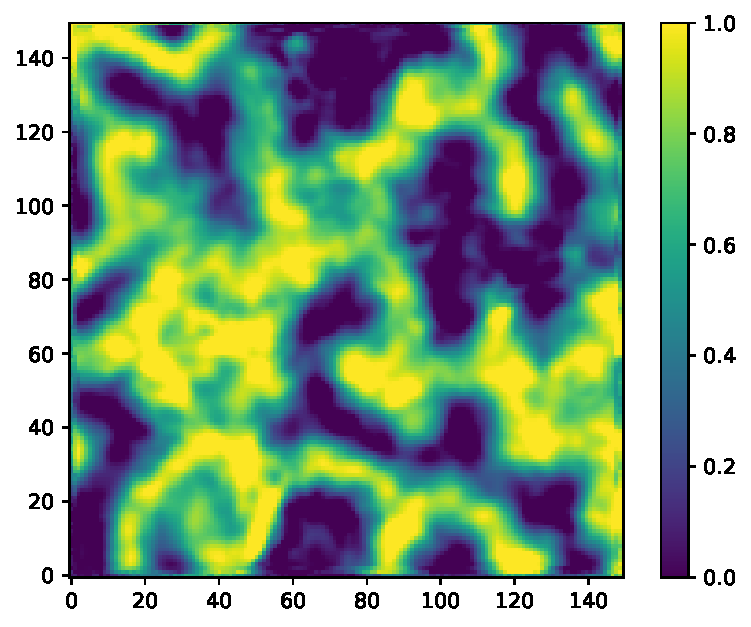
\includegraphics[height=2.5in]{figures/results/unblur/esn_barkley_u_blur_pred.pdf}
		\setcapmargin[1cm]{0.5cm}
  		\caption{Vorhersage des \textsc{ESN}}
  		\label{fig:exp_unblur_barkley_result_esn_pred}
	\end{subfigure}
	\caption{Graphische Darstellung der $u$-Variable des \textit{Barkley}-Modells für den $100$. Zeitschritt des Evaluationsdatensatzes. Oben links ist das tatsächliche Feld des Modells zu sehen. Danach folgen in Leserichtung die Vorhersagen des \textsc{NN}-Ansatzes, des \textsc{RBF}-Ansatzes und des \textsc{ESN}. Das verwendete Fernfeld ist in Abbildung \ref{fig:exp_unblur_barkley_blurred} zu sehen. }
	\label{fig:exp_unblur_barkley_result}
\end{figure} 

\begin{table}[h]
	\centering
	\captionsetup{width=0.9\linewidth}
	\begin{tabular}{cccccccc}
		\hline
		\multicolumn{1}{c}{} & \multicolumn{3}{c}{Barkley} & \multicolumn{3}{c}{Mitchell-Schaeffer}		\\
		%\cline{2-7}
		\multicolumn{1}{c}{} & NN & RBF & ESN & NN & RBF & ESN \\
		
		\hline
		
		Laufzeit [s] 	& \textbf{53} 	& 1840		& 3604				& \textbf{42}	& 1842 		& 3823 \\
		MSE 			& 0.10089		& 0.03984	& \textbf{0.02443} 	& 0.06452		& 0.03384 	& \textbf{0.02645} \\
		NRMSE 			& 0.8308		& 0.5170	& \textbf{0.4048} 	& 0.9737		& 0.7052 	& \textbf{0.6234} \\
		\hline 
	\end{tabular} 
	\caption{Vergleich der benötigten Laufzeit und des erreichten Fehlers der drei Ansätze für das \textit{Mitchell-Schaeffer}- und das \textit{Barkley}-Modell, die zu den geringsten Fehlern führen.}
	\label{tab:exp_unblur_comparison_results}
\end{table}

\FloatBarrier